\subsection{并行计算与加速比}
普通计算机执行任务计算时,大多需要按照处理流程将任务划分为多个子任务,
子任务需要等待其他依赖任务执行完毕,而HPC使用更多的资源、更多的算力来
一次执行更多的任务,解决问题的时间依赖于可用的资源、以及算法的设计。
也就是说,通过更好的硬件、更多的资源、以及更好的算法如并行计算等来提高系统的算力。
HPC中有两种数据处理模式\cite{amd_hpc}:

\begin{itemize}
    \item \textbf{串行处理}: 由CPU完成,每个CPU核心通常每次只能处理一个任务
    \item \textbf{并行处理}: 可利用多个CPU或GPU完成,
    GPU 最初是专为图形处理而设计的。
    它可在数据矩阵(如屏幕像素)中同时执行多种算术运算。
     同时在多个数据平面上工作的能力使 GPU 非常适合在机器学习 (ML) 应用任务中进行并行处理,
    如识别视频中的物体。
\end{itemize}

根据阿姆达尔定律(Amdahl's law),固定负载的计算任务在并行化之后的效率提升,
可以用以下公式来表示\cite{wiki_amdahls_law}:
$$
S_\text{latency}(s) = \frac 1 {(1 - p) + \frac p s}
$$

其中,
\begin{itemize}
    \item $S_\text{latency}$为理论加速比
    \item $s$为处理器数量
    \item $p$为可以并行处理的部分比例
\end{itemize}

阿姆达尔定律下,增加并行处理器的数目最终会达到一个极限的加速比,
受限于程序设计中的串行部分,如\cref{amdahlslaw}所示。

\begin{figure}[ht!]
    \centering
    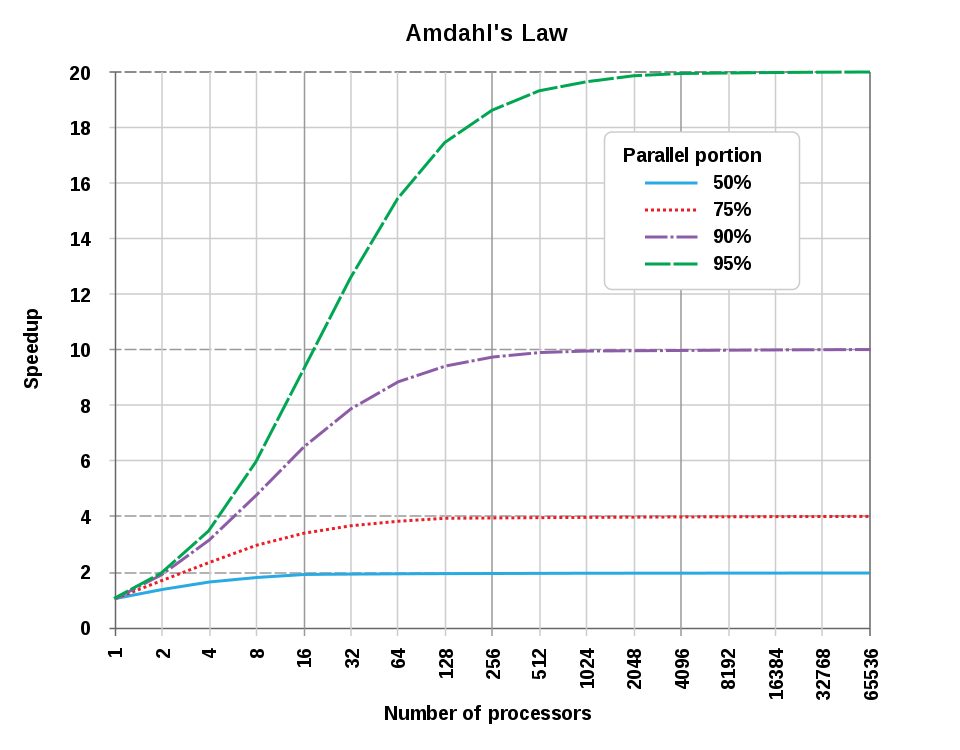
\includegraphics[width=\linewidth]{images/AmdahlsLaw.png}
    \caption{增大处理器数目并不能无限增大加速比,这取决于程序的可并行度}
    \label{amdahlslaw}
\end{figure}

阿姆达尔定律假设问题的大小是固定的,串行执行的总耗时是固定的,
但在实际问题中,一个重要的事实是,
并行计算不仅可以进行加速,
也可以为解决问题提供更大的空间,
可以处理更大规模的问题,
而其又可以拆分为更多独立的小问题来并行解决\cite{when_amdahls_law_does_not_apply}。
因此,另一个更优的模型是古斯塔夫森定律(Gustafson's law)\cite{wiki_gustafson},
它可以表示为:

\begin{align}
S &= s + p \times N \\
    &= s + (1 - s) \times N \\
    &= N + (1 - N) \times s
\end{align}

其中,
\begin{itemize}
    \item $S$为理论加速比
    \item $N$为处理器数量
    \item $s$、$p$分别为程序花费在串行和并行计算上部分所占的比例,满足$s+p=1$
\end{itemize}

根据这一定律,可以得出一个更符合实际应用的加速比与处理器关系图,
如\cref{gustafsons_law}所示。

\begin{figure}[ht!]
    \centering
    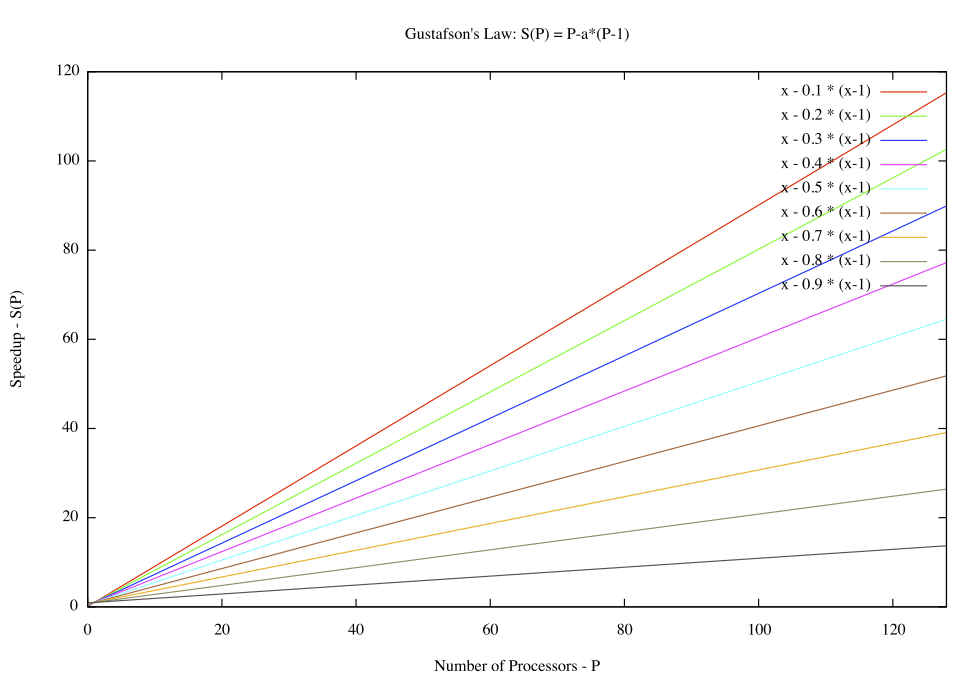
\includegraphics[width=\linewidth]{images/Gustafson.png}
    \caption{根据古斯塔夫森定律得出的计算比与处理器的关系}
    \label{gustafsons_law}
\end{figure}

\subsection{HPC系统的计算模型}
HPC系统需要使用高性能的硬件,
包括CPU、加速器、以及存储和网络设备等;
除此之外,还需要一个顶层的设计,
来决定计算负载将如何被执行。
在进行并行计算时,有两种模型,
分别是共享内存模型和分布式内存模型两种\cite{intro_cluster_computing},
参见\cref{parallel_models}。
它们的特点如\cref{parallel_model_keys}所示。

\begin{figure}[ht]
\begin{tabularx}{\textwidth}{|X|X|}
\toprule
\textbf{共享内存模型} & \textbf{分布式内存模型} \\
\midrule
\begin{itemize}
    \item 所有处理器都可以在同一地址空间访问所有内存
    \item 不同处理器可以单独运行但共享相同的内存资源
    \item 处理器对某内存地址的改变对其他所有处理器可见
\end{itemize}    &
\begin{itemize}
    \item 分布式内存模型系统需要网络通信来连接各个处理器的内存
    \item 处理器拥有单独的本地内存和地址空间,并没有全局的地址空间
    \item 每个处理器单独运行,对其本地内存的改变对其他处理器没有影响
    \item 当处理器需要访问其他处理器的数据时,需要由程序来显式进行定义,
    并可能需要进行同步处理
\end{itemize} \\
\bottomrule
\end{tabularx}
\caption{两种并行计算模型的特点}
\label{parallel_model_keys}
\end{figure}

\begin{figure}[ht!]
    \centering
    \begin{subfigure}{.5\textwidth}
        \centering
        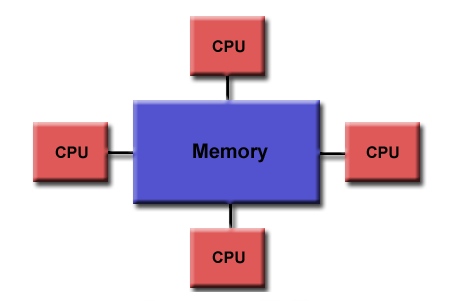
\includegraphics[width=0.9\linewidth]{images/shared-memory.png}
        \caption{共享内存模型}
    \end{subfigure}%
    \begin{subfigure}{.5\textwidth}
        \centering
        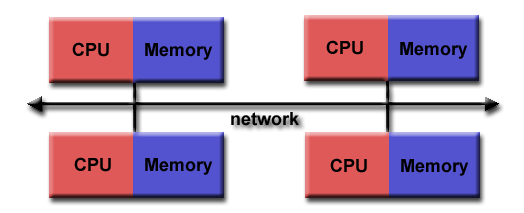
\includegraphics[width=\linewidth]{images/distributed-memory.png}
        \caption{分布式内存模型}
    \end{subfigure}
    \caption{并行计算的两种模型}
    \label{parallel_models}
\end{figure}

HPC系统有以下几种设计模式\cite{ibm_hpc}:

\begin{itemize}
    \item \textbf{并行计算}: 按照共享内存模型,
    使用成百上千的处理器进行协同计算
    \item \textbf{集群计算}: 使用相同的计算机组成集群,
    使用高速的本地网络进行互连,
    并使用中心化的任务调度和资源管理来执行计算任务。
    整个集群组成了一个HPC系统。
    \item \textbf{网格计算}: 通过网络将多个计算机连接起来,
    它们可以同处一个本地网络或者分布于不同的地理位置。
    相对于集群计算而言,网格计算可以使用不同类型的计算机,
    网格中的计算机可以向集群贡献剩余算力。
    不同网格中的计算机使用低速网络互连,
    但每个网格可以实现自治。
\end{itemize}

\subsection{硬件设施及网络拓扑}
典型的HPC集群架构如\cref{hpc_structure}所示。其中,
SMS(System Management Server)为控制节点,
通过BMC\footnote{BMC:基板管理控制器(Baseboard Management Controller),
它可以在机器未开机状态下对机器进行固件升级、查看机器设备等操作。}
网络与计算节点联通。

\begin{figure}[ht!]
    \centering
    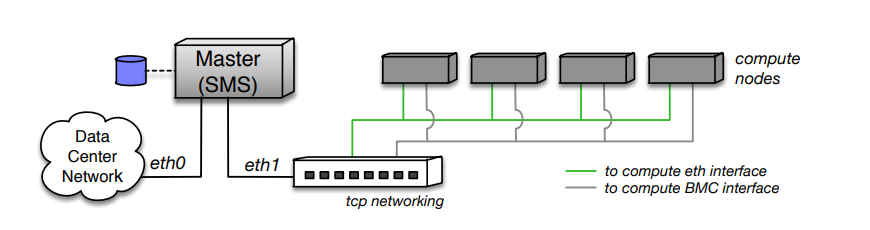
\includegraphics[width=\linewidth]{images/hpc-cluster-structure.png}
    \caption{ohpc示例的HPC集群的整体架构\cite{ohpc}}
    \label{hpc_structure}
\end{figure}

\subsubsection{高速网络}
除开以太网外,HPC集群中还可以增加高速网络来传输,
例如进行消息传递、并行文件系统传输等,
主要包含InfiniBand、Omni-Path\footnote{Omni-Path由Intel推出,
但不就宣布放弃此项技术\cite{wiki_omni_path}。}等。

InfiniBand(“无限带宽”)是一个用于高性能计算的计算机网络通信标准,
它具有极高的吞吐量和极低的延迟,
用于计算机与计算机之间的数据互连。
InfiniBand也用作服务器与存储系统之间的直接或交换互连,
以及存储系统之间的互连\cite{wiki_infiniband}。

InfiniBand高效率、低延迟,且能够支持一个子网中上千节点,
并可以通过路由几乎无限扩展。
同时,它支持RDMA (Remote Direct Memory Access)技术,
能够绕开内核直接读取数据,从而有更高吞吐量和更低延迟
\cite{infiniband_future,wiki_rdma,infiniband_eth}。

\subsection{HPC技术栈}
HPC技术栈选择较多,主要包含操作系统、集群调度、编译器等
涵盖HPC管理、编程、监控等各个维度的工具链。

\subsubsection{操作系统}
HPC几乎全部使用Linux操作系统,但大多为RH/SUSE系列,
例如劳伦斯Livermore国家实验室(LLNL)的超算使用的是给予RHEL的
TOSS(Trilab Operating system Software Stack):

\begin{itemize}
    \item Red Hat系列,包括RHEL、CentOS、Rocky Linux
    \item SUSE系列,包括SLES、Open SUSE
\end{itemize}

\subsubsection{文件系统}
HPC集群中一些常用的文件系统包括:

\begin{itemize}
    \item NFS: 中小型集群中使用较多
    \item GPFS: 高性能的专有并行文件系统
    \item Lustre: 高性能的开源并行文件系统
\end{itemize}


\subsubsection{操作系统置备及集群管理}
集群管理软件负责初始化以及维护裸金属服务器或者虚拟机,
例如操作系统置备(OS Provision)、固件更新、软件管理、文件分发等,
对于大规模集群来说,这是十分有必要的。
尽管这类软件是为HPC而开发的,但也可以用来管理其他类型的集群,
例如Kubernetes集群。

主要有以下两种选择:

\begin{itemize}
    \item Warewulf: 轻量级、无状态的管理软件
    \item xCAT: 比Warewulf功能更强大,但也更复杂一些。
    2018 Top500排名第1和第二的Summit、Sierra均采取xCAT进行管理,
    并为IBM的官方HPC管理软件
\end{itemize}

\subsubsection{资源管理/作业调度}
分布式资源管理系统(D-RMS)负责控制HPC集群中硬件资源的使用,
包括CPU、内存、磁盘、带宽等,
用户提交任务后,D-RMS将选择以最优的方式进行任务分配和执行
\cite{comparative_drms,hpc_wiki_batch_scheduler},
主要包括以下几种:

\begin{itemize}
    \item Portable Batch Systems(PBS): OpenPBS业内使用最广泛的集群调度系统,它还有商用版本PBSPro
    \item SLURM: 另一款开源调度系统
    \item Platform Load Sharing Facility(LSF): IBM Spectrum LSF社区版
    \item Grid Engine: 支持网格计算的资源和负载管理系统,最初由Sun创建\cite{wiki_grid_engine}
\end{itemize}

除了传统的HPC调度系统,
Kubernetes也是一种分布式资源管理和调度系统,
但它从设计上与传统HPC调度系统有一定的差别,
分别适合不同的场景\cite{choose_k8s_lsf}。

\subsubsection{编译器及开发工具}
HPC任务通常由c/c++/fortran编写,
代码需要在目标平台上进行编译后执行,
因此需要安装相应的编译器。
一些商用编译器还特别对并行计算代码进行优化。
主要有:

\begin{itemize}
    \item GNU编译器族: gcc/g++等
    \item llvm编译器族: clang/clang++等
    \item ARM平台c/c++/fortran编译器\cite{arm_hpc_tools}
    \item 商用编译器,如Intel编译器、PGI编译器、PathScale等 
    \item 工具链: autoconf、automake、cmake、python等 
    \item 其他: Valgrind内存调试器、Spack包管理
\end{itemize}

\subsubsection{性能分析工具}
性能分析工具用来分析HPC应用的表现及调优,
从而能够更好地利用资源。例如:

\begin{itemize}
    \item BSC工具集:Paraver、Dimemas、Extrae等
    \item OSU Micro-benchmarks、gperftools、perf等
\end{itemize}

\subsubsection{开发库}
HPC应用编译及运行需要的一些软件库:

\begin{itemize}
    \item 并行I/O库: 如ADIOS、HDF5、NetCDF、PnetCDF等
    \item 线性代数库: 如PETSc、BLAS、Lapack、SuperLU等
    \item 偏微分方程库: 如PETSc、Trilinos等
    \item 图算法库: 如PBGL、Giraph等
    \item 网格分解: 如METIS、ParMETIS、Zoltan
    \item 可视化: 如VTK、Gnuplot、Matplotlib、ParaView等
    \item 消息传递: 分布式内存模型下需要,主要是MPI\footnote{Message Passing Interface(MPI)是一个跨语言的通讯协议,
    用于编写并行计算机。支持点对点和广播。
    MPI是一个信息传递应用程序接口,包括协议和和语义说明,他们指明其如何在各种实现中发挥其特性。MPI的目标是高性能,大规模性,和可移植性。
    MPI在今天仍为高性能计算的主要模型\cite{wiki_mpi}。}
    包括OpenMPI、MPICH、Intel MPI等实现
    \item 多线程: 共享内存模式下需要,主要是OpenMP、Pthreads等
\end{itemize}

\subsubsection{加速器相关}
HPC中需要用到GPU等进行加速,
而GPU本身是为图形处理而设计的,
需要使用一些框架来进行异构计算编程,
主要包括:

\begin{itemize}
    \item CUDA: 适用于NVIDIA显卡的专有GPU编程工具包
    \item OpenCL: 开放计算语言(Open Computing Language),是一个异构编程规范
    \item C++ AMP: C++加速大规模并行(C++ Accelerated Massive Parallelism)
    是由微软开发的C++编译器和扩展集,使得C++应用程序可以利用GPU等进行加速\cite{c++_amp}
    \item OpenACC: 开源加速器(Open Accelerators)是一个是为了简化异构计算(CPU/GPU)系统的并行编程的并行计算编程标准。
\end{itemize}